%\setchapterimage{fig_01.png}
\chapter*{TD \arabic{cptTD} \\ 
Stabilisateur actif d'image   -- \ifprof Corrigé \else Sujet \fi}
\addcontentsline{toc}{section}{TD \arabic{cptTD} :  Stabilisateur actif d'image  -- \ifprof Corrigé \else Sujet \fi}

\iflivret \stepcounter{cptTD} \else
\ifprof  \stepcounter{cptTD} \else \fi
\fi

\setcounter{question}{0}
\marginnote{Mines Ponts 2018 -- PSI}
\marginnote{
\UPSTIcompetence[2]{C1-01}
\UPSTIcompetence[2]{C2-03}}

\begin{marginfigure}
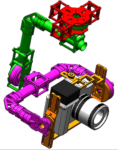
\includegraphics[width=.8\linewidth]{Cy_02_Ch_01_TD_02_Stabilisateur}
\end{marginfigure}

\subsection*{Mise en situation}
\ifprof
\else
On s'intéresse à une nacelle active de caméra. Ce système de stabilisation, nommé CAM-GYR, permet de s'assurer que quelque soit l'orientation du porteur (caméraman), l'axe vertical de la caméra et toujours parallèle à la direction de la pesanteur. 
Le système est équipé de 3 moteurs permettant d'ajuster le roulis, le tangage et le lacet. On s'intéresse ici uniquement à la stabilisation de l'axe de tangage. 

\begin{center}
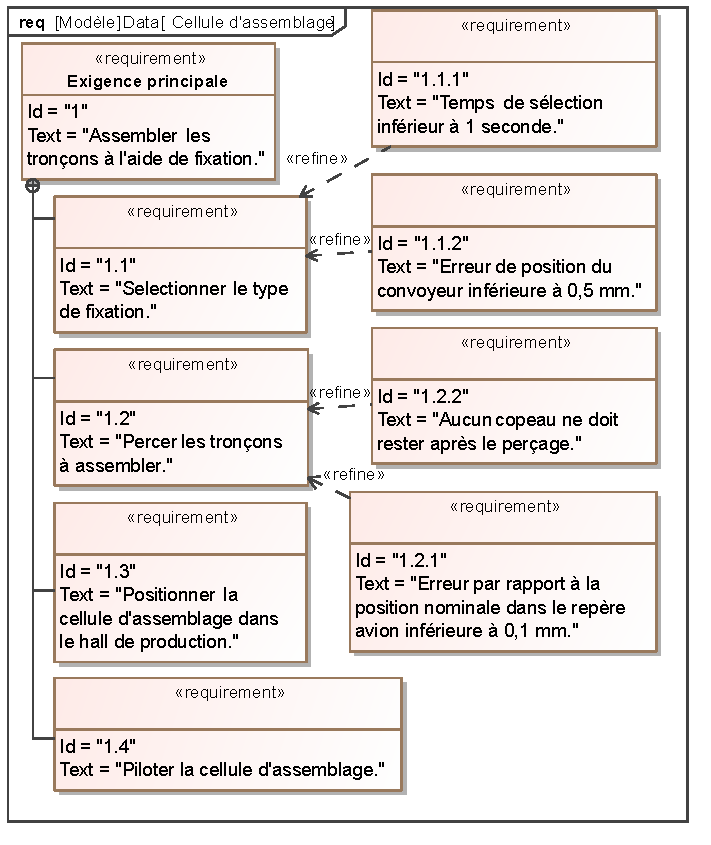
\includegraphics[width=\linewidth]{Exigences}
\end{center}
\fi
\begin{obj}
Vérifier l'exigence 1.1 « déplacer la caméra ». %Proposer un réglage d’un axe suivant plusieurs modes de fonctionnement.
\end{obj}



\subsection*{Travail demandé}
\ifprof
\else
On considère un modèle de l’axe de tangage sans perturbation et qui reçoit des consignes assez rapides modélisées par
des échelons.
L’ensemble \{moteur, charge\} ne présente pas de réducteur. Il est modélisé par un ensemble en série de deux fonctions
de transfert :
\begin{itemize}
\item un gain pur de valeur $K_m$;% (La valeur KmT du DOCUMENT D4 est notée Km dans cette partie) ;
\item une fonction de transfert du premier ordre de gain statique $A$ et de constante de temps $\tau_m$.
\end{itemize}
Cet ensemble présente comme entrée la commande du moteur $\text{com(t)}$ et comme sortie la vitesse angulaire de rotation
du moteur $\omega_m(t)$. Le réglage retenu est tel que $K_m A = 1$. \textbf{Le retour $K_D$ agit par un sommateur.}
Dans cette étude, $A_i(p)=1$.
%Enfin, lors de mouvement brusque de la caméra, on souhaite arriver progressivement sur la scène finale sans choc ni oscillation mais avec précision. Ainsi, la commande peut être modifiée selon 3 cas de fonctionnements : 
%\begin{itemize}
%\item $A_1(p)=1$ : pas de traitement;
%\item $A_2(p)= \dfrac{1}{\tau_0 p} \left( 1-e^{-\tau_0 p}\right)$ : fonction rampe de pente 1 pour rejoindre la valeur finale;
%\item $A_3(p)= \dfrac{1}{1+\tau_0 p}$ : fonction de transfert du  premier ordre de constante de temps $\tau$ (filtre passe-bas).
%\end{itemize}
\begin{figure}[H]
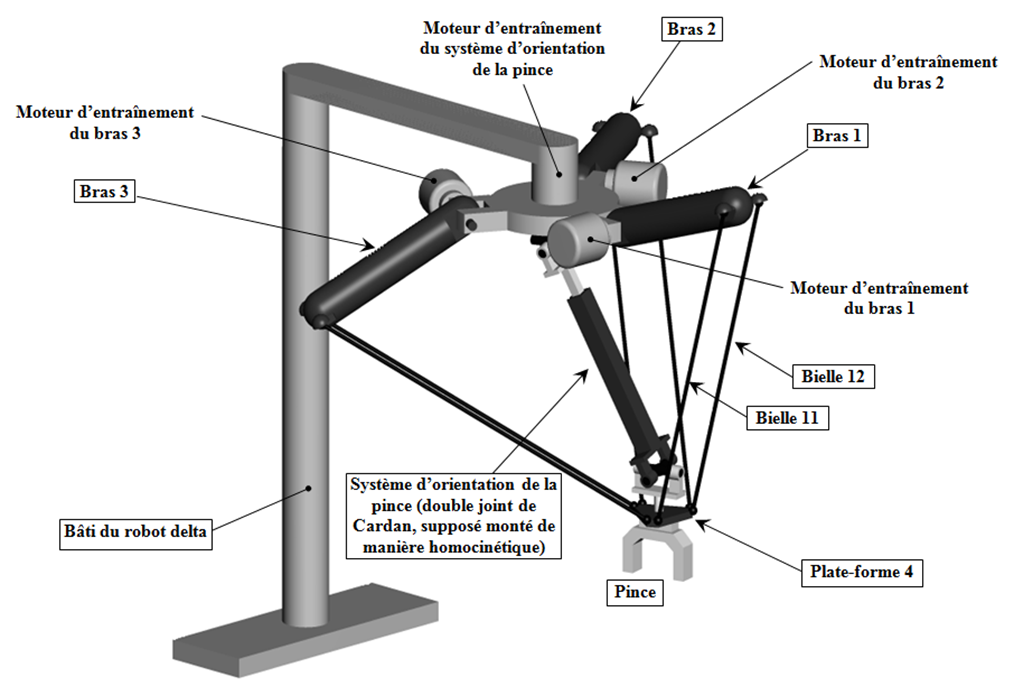
\includegraphics[width=.8\linewidth]{fig_01}

\caption{Modèle 1 de l’axe de tangage.}
\end{figure}

\fi

\question{Avec $K_m A = 1$, calculer la fonction de transfert en boucle ouverte (FTBO) et la fonction de transfert
en boucle fermée (FTBF) du schéma (modèle 1).}
\ifprof
\begin{corrige}
\textbf{Attention au signe du comparateur de la boucle inbriquée !}

On définit la FTBO par $\text{FTBO}(p)=\dfrac{\varepsilon(p)}{\text{Mes}\varphi(p)}$ avec $\varepsilon(p)$ la sortie du premier comparateur.

On a d'une part $G(p)=\dfrac{\dfrac{K_m A}{1+\tau_m p}}{1-\dfrac{K_m A K_D }{1+\tau_m p}}= \dfrac{K_m A}{1+\tau_m p-K_m A K_D }$.
On a alors $\text{FTBO}(p)=\dfrac{K_m A K_P}{p\left(1+\tau_m p-K_m A K_D \right)}$. 

Si on définit la FTBF par $\text{FTBF(p)}=\dfrac{\varphi(p)}{\varphi^{\star}(p)}$, on a 
$\text{FTBF(p)}=A_i(p)\dfrac{\dfrac{K_m A K_P}{p\left(1+\tau_m p-K_m A K_D \right)}}{1+\dfrac{K_m A K_P}{p\left(1+\tau_m p-K_m A K_D \right)}}$ 

$=A_i(p)\dfrac{K_m A K_P}{p\left(1+\tau_m p-K_m A K_D \right)+K_m A K_P}$.

Au final, 
$\text{FTBO}(p)=\dfrac{ K_P}{p\left(1+\tau_m p-K_D \right)}$ et 
$\text{FTBF}(p)=A_i(p)\dfrac{K_P}{p\left(1+\tau_m p- K_D \right)+K_P}$.
\end{corrige}
\else
\fi

Dans un premier temps en mode pilotage, on s’intéresse au comportement de l’axe de tangage sans le filtre passe bas :
$A_1(p)=1$.

\question{Quelle est la valeur maximale de $K_D$ pour que la commande de l’axe de tangage soit strictement
stable ? Préciser le(s) critère(s) de stabilité appliqué(s).}
\ifprof
\begin{corrige}
Pour que le système soit stable, tous les coefficients du dénominateur $D(p)$ de la FTBF doivent être de même signe (ainsi toutes les racines sont à partie réelle négative). On a 
$D(p)=p\left(1+\tau_m p- K_D \right)+K_P = \tau_m p^2 p+ \left(1-K_D \right)p +K_P$ et donc nécessairement, 
$1-K_D >0$ et $K_D < 1$.
\end{corrige}
\else
\fi

\ifprof
\else
En accord avec les résultats précédents, on fixe $K_D = 0,5$ et $\tau_m = \SI{0,2}{s}$.
Dans un premier temps on impose $K_P = \SI{10}{s^{-1}}$.
\fi
%
%La figure temporelle ci-dessous propose une réponse du système avec un filtre passe
%bas de constante de temps 2 secondes et de gain égal à 1 ($A_i(p)=\dfrac{1}{1+\tau_0 p}$).%'[i=3].
%
%\begin{center}
%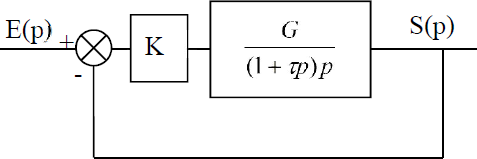
\includegraphics[width=\linewidth]{fig_02}
%\end{center}


\question{Lorsque $A_i(p)=1$, le comportement est-il compatible avec l’exigence 1.1.1 «~Maîtriser les déplacements~» ? }
\ifprof
\begin{corrige}
On a : $\text{FTBF}(p)=
\dfrac{K_P}{p+\tau_m p^2- K_Dp +K_P}$ 
$=\dfrac{K_P}{\dfrac{\tau_m}{K_p} p^2 + p\dfrac{1- K_D}{K_P} +1}$.

On a alors $\omega_0 = \sqrt{\dfrac{K_P}{\tau_m}}$ et $\xi = \dfrac{1- K_D}{K_P} \dfrac{\sqrt{\dfrac{K_P}{\tau_m}}}{2}= \dfrac{1- K_D}{2\sqrt{K_P \tau_m}}= \dfrac{0,5}{2\sqrt{2}} <1$. Il y a donc du dépassement. L'exigence n'est pas vérifiée. 
\end{corrige}
\else
\fi

\ifprof
\else

Dans un second temps on se place en mode stabilisation. On s’intéresse toujours au comportement de l’axe de
tangage mais sans le filtre passe bas ($A_1(p)=1$).
On considère ici que la consigne est constante donc $\varphi^*_a(t)=0$. Une perturbation $\text{Pe(p)}$ agit au niveau de l’ensemble (moteur, charge) modélisée sur le schéma bloc (Modèle 2). On appelle $\text{Com(p)}$ la transformée de Laplace de la commande du moteur $\text{com(t)}$.

\begin{figure}[H]
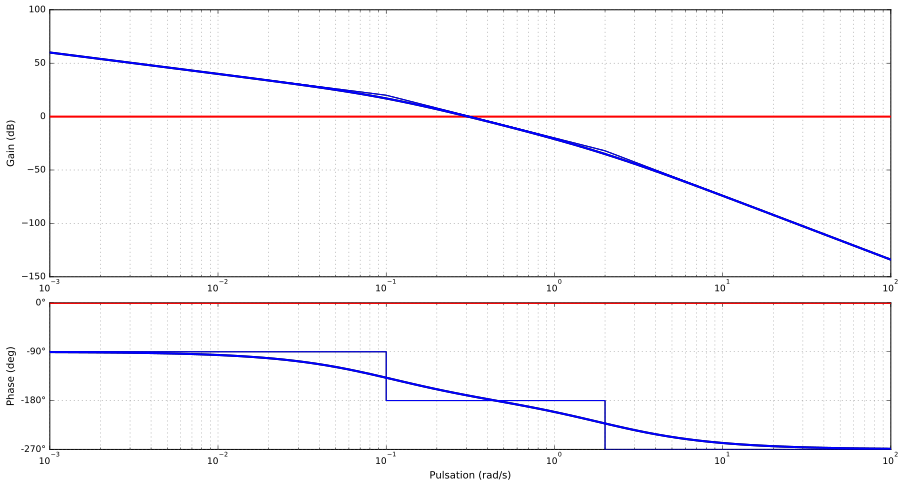
\includegraphics[width=.8\linewidth]{fig_03}

\caption{Modèle 2 de l’axe de tangage.}
\end{figure}
\fi

\question{Avec le « modèle 2 » calculer la fonction de transfert $\text{Stab}(p)=\dfrac{\text{Com}(p)}{\text{Pe}(p)}$ qui lie la commande à la perturbation.}% Conseil de résolution : calculer $\varepsilon_1$ en fonction de $\text{Pe}(p)$, $\text{Com}(p)$ et des fonctions de transfert utiles, puis calculer $\varepsilon_2$ en fonction de $\varepsilon_1$ et des fonctions de transfert utiles, puis $\varepsilon_3$ en fonction de $\varepsilon_1$, $\varepsilon_2$ et des fonctions de transfert utiles et enfin en déduire $\text{Stab}(p)=\dfrac{\text{Com}(p)}{\text{Pe}(p)}$.}
\ifprof
\begin{corrige}
On a $\varepsilon_2(p) = -\text{Mes}\left( \varphi(p)\right) = -\varphi(p) = -\varepsilon_1(p)\dfrac{1}{p}$. 
Par ailleurs, $\varepsilon_1(p)=\text{Pe}(p)+\varepsilon_3(p)\dfrac{AK_m}{1+\tau_m p}$. 
Enfin, $\varepsilon_3(p)=K_P\varepsilon_2(p)+K_D \varepsilon_1(p)$ $\Leftrightarrow \varepsilon_3(p)=\varepsilon_1(p)\left(K_D-\dfrac{K_P}{p} \right)$
$\Leftrightarrow \varepsilon_1(p) =\varepsilon_3(p)\dfrac{1}{K_D -\dfrac{K_P}{p} }$. 

On a donc  $\varepsilon_3(p)\dfrac{1}{K_D -\dfrac{K_P}{p}}=\text{Pe}(p)+\varepsilon_3(p)\dfrac{AK_m}{1+\tau_m p} $ $\Leftrightarrow \varepsilon_3(p)\left(\dfrac{p}{pK_D-K_P } -\dfrac{AK_m}{1+\tau_m p}\right)=\text{Pe}(p) $ 

$\Leftrightarrow \varepsilon_3(p)\dfrac{p\left(1+\tau_m p \right) - AK_m \left( pK_D-K_P\right) }{\left(pK_D-K_P \right) \left(1+\tau_m p\right)}=\text{Pe}(p) $.

On a donc $\text{Stab}(p)=\dfrac{\text{Com}(p)}{\text{Pe}(p)}=\dfrac{\left(pK_D-K_P \right) \left(1+\tau_m p\right)}{p\left(1+\tau_m p \right) - AK_m \left( pK_D-K_P\right) }$.


\end{corrige}
\else
\fi

\question{\label{q28}Avec le modèle 2 et une entrée $\text{Pe}(p)$ échelon unitaire, déterminer la limite quand t tend vers
l’infini de la commande : $\text{com}(t)$. Quel sens physique donner à ce résultat ?}
\ifprof
\begin{corrige}
On a $\lim\limits_{t\to\infty}\text{com}(t) = \lim\limits_{p\to 0}p\text{Com}(p)$ 
$=\lim\limits_{p\to 0}p\text{Stab}(p)\text{Pe}(p)$ 

  $= \lim\limits_{p\to 0}p\dfrac{1}{p} \dfrac{\left(pK_D-K_P \right) \left(1+\tau_m p\right)}{p\left(1+\tau_m p \right) - AK_m \left( pK_D-K_P\right) }$
   $= \lim\limits_{p\to 0} \dfrac{-K_P }{  AK_m  K_P }=-1$ si $AK_m=1$.
  
  Ainsi, pour une perturbation angulaire dans un autre sens, le système commande les moteurs avec une consigne dans le sens opposé. 
\end{corrige}
\else
\fi

\question{Avec le modèle 2 déterminer la FTBO $\dfrac{\text{Mes}\varphi(p)}{\varepsilon_2(p)}$ de ce schéma puis calculer la fonction de transfert liant la perturbation et la sortie $\text{Pert}(p)=\dfrac{\varphi(p)}{\text{Pe}(p)}$.}
\ifprof
\begin{corrige}

On a  $\dfrac{\text{Mes}\varphi(p)}{\varepsilon_2(p)} = \dfrac{K_m A K_P}{p\left(1+\tau_m p-K_m A K_D \right)}$ (c'est la même que pour le premier modèle).

On a vu que  $\varepsilon_2(p) = -\varphi(p) = -\varepsilon_1(p)\dfrac{1}{p}$, $\varepsilon_1(p)=\text{Pe}(p)+\varepsilon_3(p)\dfrac{AK_m}{1+\tau_m p}$ et $\varepsilon_3(p)=\varepsilon_1(p)\left(K_D-\dfrac{K_P}{p} \right)$. 

En conséquences, $\varepsilon_1(p)=\text{Pe}(p)+\varepsilon_3(p)\dfrac{AK_m}{1+\tau_m p} \Longleftrightarrow 
\varepsilon_1(p)=\text{Pe}(p)+\varepsilon_1(p)\left(K_D-\dfrac{K_P}{p} \right)\dfrac{AK_m}{1+\tau_m p}$

$ \Leftrightarrow 
\varepsilon_1(p)\left( 1+\left(\dfrac{K_P}{p}-K_D \right)\dfrac{AK_m}{1+\tau_m p}\right)=\text{Pe}(p)$
$ \Leftrightarrow 
p\varphi(p)\left( 1+\left(\dfrac{K_P}{p}-K_D \right)\dfrac{AK_m}{1+\tau_m p}\right)=\text{Pe}(p)$

et donc $\text{Pert}(p)=\dfrac{1}{p\left( 1+\left(\dfrac{K_P}{p}-K_D \right)\dfrac{AK_m}{1+\tau_m p}\right)}$
$=\dfrac{1}{p\left( 1+\dfrac{K_P-pK_D}{p}\dfrac{AK_m}{1+\tau_m p}\right)}$
$=\dfrac{1+\tau_m p}{p \left(1+\tau_m p\right)+\left(K_P-pK_D\right)AK_m}$.



\end{corrige}
\else
\fi



\question{Déterminer la valeur lorsque $t$ tend vers l’infini de la réponse temporelle de ce système à une
perturbation de type échelon unitaire. Quel sens physique donner à ce résultat ?}
\ifprof
\begin{corrige}
On a $\lim\limits_{t\to\infty}\varphi(t) = \lim\limits_{p\to 0}p\Phi(p)$ 
$=\lim\limits_{p\to 0}p\text{Pert}(p)\text{Pe}(p)$
  $= \lim\limits_{p\to 0}p\dfrac{1}{p} \dfrac{1+\tau_m p}{p \left(1+\tau_m p\right)+\left(K_P-pK_D\right)AK_m}$
  
  $= \lim\limits_{p\to 0}\dfrac{1}{K_PAK_m} =\dfrac{1}{K_P}=0,1\degres$.
  
Le système n'est pas précis s'il y a une perturbation échelon. 
\end{corrige}
\else
\fi

\question{On désire une marge de gain de $M_G \geq \SI{5}{dB}$ et une marge de phase $M\varphi \geq 20\degres$ (exigence 1.1.3 « Stabilité de la commande »). Déterminer la valeur maximale de $K_P$ en utilisant les données ci-dessous.}
% (OU 40 ?degres)




%\begin{center}
%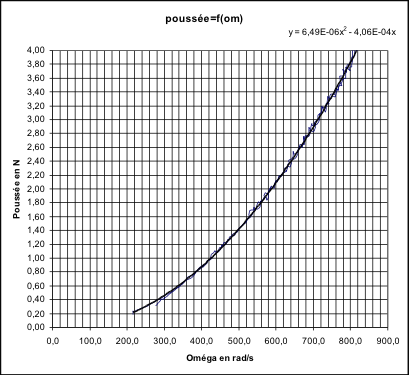
\includegraphics[width=\linewidth]{fig_04}
%\end{center}
\ifprof
\begin{corrige}
Pour une marge  de de phase de 20\degres, la phase doit être de $-160\degres$ lorsque le gain est nul. Or en $-160\degres$ le gain est de \SI{-3}{dB}. Pour respecter la marge de phase, il faut donc déterminer $K_P$ tel que $20\log K_P = 3$ soit $K_P < 10^{\dfrac{3}{20}}\simeq1,41 $.

Le système étant d'ordre 2, la marge de gain sera forcément infinie.
\end{corrige}
\else


On note $F(\omega)= \dfrac{2}{j\omega \left(1+0,4 j\omega \right)}$.

\footnotesize
\begin{center}
\begin{tabular}{llllll}
\hline
$\omega$ (rad/s) & 1 & 2,5 & 5 & 7 & 10 \\ \hline
$\text{Arg}\left(F(\omega)\right)$  & $-112\degres$ & $-135\degres$ & $-153\degres$ & $-160\degres$ & $-166\degres$ \\ 
$20 \log \left| F(\omega)\right|$ & \SI{5,4}{dB} & \SI{3}{dB} & \SI{-1}{dB} & \SI{-3}{dB} & \SI{-6,2}{dB} \\ \hline
\end{tabular}
\end{center}
\normalsize

\fi

\ifprof
\else
Le figure suivante (droite) présente la réponse temporelle de l’axe de tangage à une perturbation sinusoïdale (due par
exemple au vent qui crée un balancement de la GYRCAM) (ordonnée en degrés).

\begin{figure*}
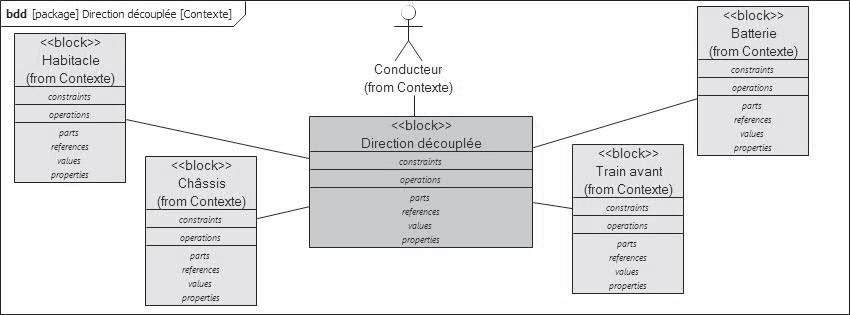
\includegraphics[width=.45\linewidth]{fig_05}\hfill
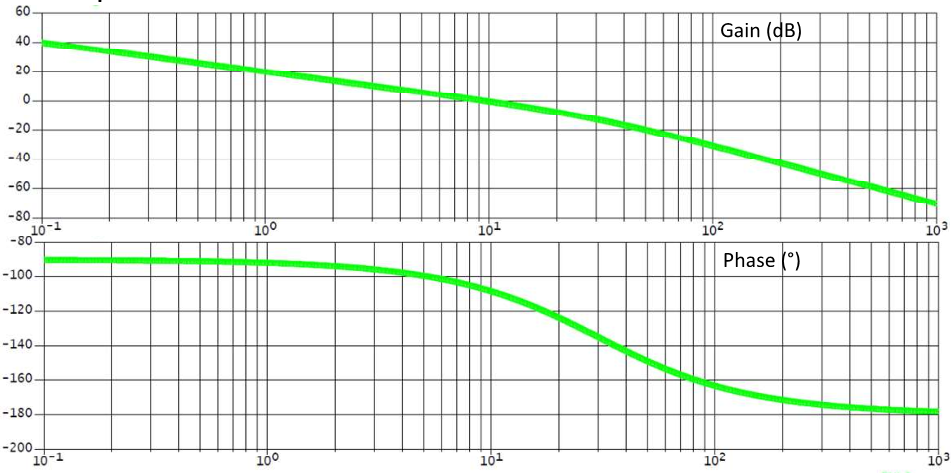
\includegraphics[width=.45\linewidth]{fig_06}
\end{figure*}

\fi

\question{Analyser ce tracé par rapport à l’exigence 1.1.2 « Perturbations » et justifier le
tracé de Com(t) relativement à Pe(t) en utilisant le résultat de la question~\ref{q28}.}
\ifprof
\begin{corrige}
La commande s'oppose à la perturbation (comme évoqué question \ref{q28}). Le stabilisateur a au final un mouvement sinusoïdal dont les valeurs maximales et minimales sont voisines de 0,1\degres et $-0,1\degres$. 
\end{corrige}
\else
\fi
\ifprof
\else
Afin d’améliorer le comportement, un autre réglage a été effectué (voir figure précédente -- droite).

%\begin{center}
%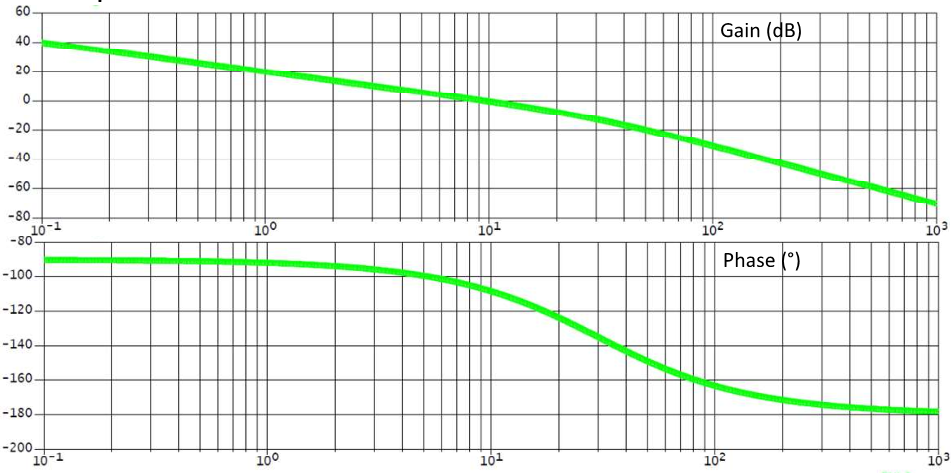
\includegraphics[width=\linewidth]{fig_06}
%\end{center}
\fi


\question{Analyser comparativement ce nouveau tracé.}% Quel(s) réglage(s) ont été fait(s) ? Quelle est l’amélioration principale obtenue ?}
\ifprof
\begin{corrige}
Dans ce cas, les mouvements du porteur sont inférieurs à 0,1 degres (en valeur absolue).
\end{corrige}
\else
\fi


\subsection*{Synthèse}
\question{En utilisant la figure suivante, faire le bilan des travaux réalisés. Quel bilan faire au vu des écarts observés entre les performances obtenues et les performances modélisées. }
\ifprof
\begin{corrige}~\\
\begin{center}
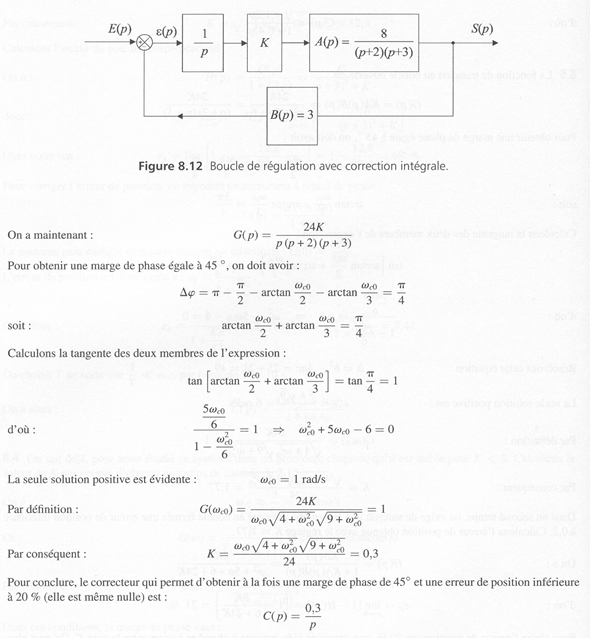
\includegraphics[width=.75\linewidth]{cor_02}
\end{center}
\end{corrige}
\else
\begin{center}
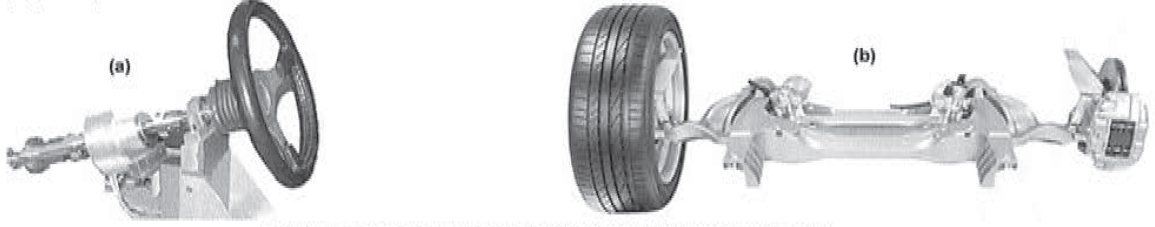
\includegraphics[width=\linewidth]{fig_07}
\end{center}
\fi

\ifcolle
\else
\ifprof
\else
\marginnote[-15cm]{
\begin{solution}
\begin{enumerate}
\item $\text{FTBO}(p)=\dfrac{ K_P}{p\left(1+\tau_m p-K_D \right)}$ et $\text{FTBF}(p)=A_i(p)\dfrac{K_P}{p\left(1+\tau_m p- K_D \right)+K_P}$.
\item $K_D < 1$.
\item 
\item $\text{Stab}(p)=\dfrac{\left(pK_D-K_P \right) \left(1+\tau_m p\right)}{p\left(1+\tau_m p \right) - AK_m \left( pK_D-K_P\right) }$.
\item $\lim\limits_{t\to\infty}\text{com}(t)=-1$.
\item $\dfrac{\text{Mes}\varphi(p)}{\varepsilon_2(p)} = \dfrac{K_m A K_P}{p\left(1+\tau_m p-K_m A K_D \right)}$  et $\text{Pert}(p)=\dfrac{1+\tau_m p}{p \left(1+\tau_m p\right)+\left(K_P-pK_D\right)AK_m}$.
\item $\lim\limits_{t\to\infty}\varphi(t) = 0,1\degres$.
\item $K_P < 1,41 $.
\item .
\item .
\end{enumerate}
\end{solution}}
\fi
\fi
